%%%%%%%%%%%%%%%%%%%%%%%%%% lecture-1
%\begin{frame}
%  \frametitle{lecture-1 主要内容}
%  \tableofcontents[hideallsubsections]
%\end{frame}

\section{课程介绍}

\begin{frame}[shrink]{课程内容}
\begin{itemize}
	%\setlength{\itemsep}{.5cm}
	\item 计算机导论:了解计算机的基本知识;掌握计算机操作基本技能。
	\item 程序设计:掌握结构化程序设计方法, 训练程序逻辑思维能力。会读、会编、会调试C语言程序。
	\item 学习方法:线上、线下相结合。课堂笔记, 认真完成上机练习作业, 鼓励大量编程练习。
	\item 教材
	\begin{itemize}
		\item 大学计算机,龚尚福, 贾澎涛,西安电子科技大学出版社
		\item C程序设计第五版, 谭浩强,清华大学出版社
	\end{itemize}
	\item 智慧教育平台(使用Chrome浏览器): 
	\href{https://cvnis.xidian.edu.cn/}{ https://cvnis.xidian.edu.cn/}
	\item 线上参考课程资源链接:
	%\href{run:./online resource.pdf}{online resource.pdf}
	\href{./online resource.pdf}{online resource.pdf} % 可以不使用run
\end{itemize}
\end{frame}

\begin{frame}{线上导论部分学习内容}
\begin{enumerate}
	\setlength{\itemsep}{.8cm}
	\item 计算机历史、现状、发展趋势与前沿技术概述
	\item 计算机体系结构及其编码方式
	\item 计算机组成与软件系统
	\item 计算机应用实践
\end{enumerate}
\end{frame}

\begin{frame}{考核}
\begin{enumerate}
	\setlength{\itemsep}{.5cm}
	\item 平时成绩: 10\%~根据上机练习作业成绩考核。
	\item 导论部分: 20\%~结合线上资源, 自学字处理软件。总结知识点,撰写课程学习报告。
	\item 期中考试: 30\%~根据机试系统给出的题目编写程序,通过调试得到正确结果并通过\textbf{机试系统提交}。
	\item 期末考试: 40\%~根据机试系统给出的题目编写程序,通过调试得到正确结果并通过\textbf{机试系统提交}。
\end{enumerate}
\end{frame}

\section{导论简介}

\begin{frame}{计算机导论主要内容}
\textbf{总体要求: 了解计算机的基本知识; 掌握计算机操作基本技能。}\\
\begin{itemize}
	\item 计算机系统组成
	\item 计算机工作原理
	\item 操作系统
	\item 字处理: Microsoft Word
	\item 电子表格: Microsoft Excel
	\item 演示文稿: Microsoft PowerPoint
\end{itemize}
\end{frame}

\begin{frame}{计算机工作原理}
\textbf{工作原理: ``存储程序'' + ``程序控制''}
\begin{enumerate}
	\item 以\textbf{二进制}形式表示数据和指令
	\item 将程序存入存储器中,由控制器自动读取并执行
	\item 外部存储器存储的程序和所需数据$\implies$计算机内存$\implies$在程序控制下由CPU周而复始地取出指令、分析指令、执行指令$\implies$操作完成。	
\end{enumerate}
\centering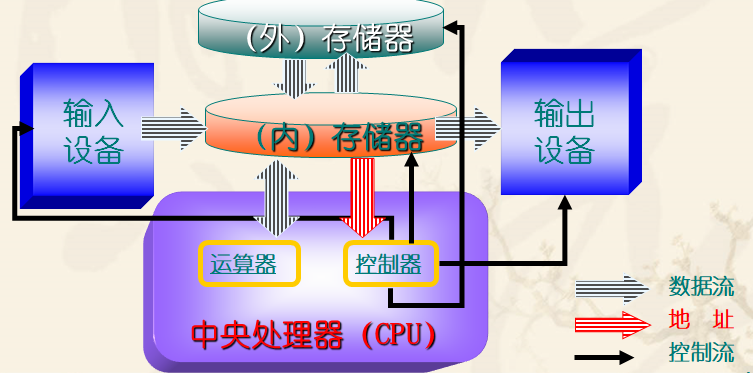
\includegraphics[scale=0.25]{hframe}
\end{frame}

\begin{frame}{十进制与二进制}
\vspace{-1cm}
\begin{align*}
&\textcolor{red}{\text{十进制: 以10为底的幂展开式:}}\\
&(123)_{10}=1\times 10^2+2\times 10^1+3\times 10^0; \\
&\textcolor{blue}{\text{自低到高各位数(除10取余至商为0): }3=123\%10,~2=123/10\%10=12\%10,}\\
&\textcolor{blue}{1=123/10/10\%10=1\%10}\\
&\textcolor{red}{\text{二进制: 以2为底的幂展开式:}}\\
&(77)_{10}=(0100\quad 1101)_{2}=0\times 2^7+1\times 2^6+0\times 2^5+0\times 2^4\\
&\qquad +1\times 2^3+1\times 2^2+0\times 2^1+1\times 2^0\\
&\textcolor{blue}{\text{自低到高各位数(除2取余至商为0): }1=77\%2,~0=77/2\%2=38\%2}\\
&\textcolor{blue}{~1=77/2/2\%2=38\%2,~1=77/2/2/2\%2=38/2\%2=19\%2,\cdots,}\\
&~\textcolor{blue}{0=77/2/2/2/2/2/2\%2=1,~0=77/2/2/2/2/2/2/2\%2=0}\\
\end{align*}
\end{frame}

\begin{frame}[shrink]
\frametitle{10进制、2进制、16进制的幂展开式}
\vspace{-0.5cm}
\begin{align*}
(D)_{10}&=D_{n-1}\times 10^{n-1}+D_{n-2}\times 10^{n-2}+\cdots+D_{1}\times 10^{1}+D_{0}\times 10^{0}\\
&+D_{-1}\times 10^{-1}+D_{-2}\times 10^{-2}+\cdots+D_{-m+1}\times 10^{-m+1}+D_{-m}\times 10^{-m}\\
&\\
(B)_{2}&=B_{n-1}\times 2^{n-1}+B_{n-2}\times 2^{n-2}+\cdots+B_{1}\times 2^{1}+B_{0}\times 2^{0}\\
&+B_{-1}\times 2^{-1}+B_{-2}\times 2^{-2}+\cdots+B_{-m+1}\times 2^{-m+1}+B_{-m}\times 2^{-m}\\
&\\
(H)_{16}&=H_{n-1}\times 16^{n-1}+H_{n-2}\times 16^{n-2}+\cdots+H_{1}\times 16^{1}+H_{0}\times 16^{0}\\
&+H_{-1}\times 16^{-1}+H_{-2}\times 16^{-2}+\cdots+16_{-m+1}\times 16^{-m+1}+H_{-m}\times 16^{-m}
\end{align*}
\end{frame}

\begin{frame}{进制对照表}
\centering
\begin{tabular}{|>{\columncolor{yellow}}c|c|c||>{\columncolor{yellow}}c|c|c|}
	\hline 
	十进制 & 二进制 & 十六进制 & 十进制 & 二进制 & 十六进制 \\ 
	\hline 
	0 & 0000 &  0 & 8 & 1000  & 8 \\ 
	\hline 
	1 & 0001 &  1 & 9 & 1001  & 9 \\ 
	\hline 
	2 & 0010 &  2 & 10 & 1010  & A \\ 
	\hline 
	3 & 0011 &  3 & 11 & 1011  & B \\ 
	\hline 
	4 & 0100 &  4 & 12 & 1100  & C \\ 
	\hline 
	5 & 0101 &  5 & 13 & 1101  & D \\ 
	\hline 
	6 & 0110 &  6 & 14 & 1110  & E \\ 
	\hline 
	7 & 0111 &  7 & 15 & 1111  & F \\ 
	\hline 
\end{tabular} 
\end{frame}

\begin{frame}{十进制、二进制与十六进制举例}
\vspace{-0.5cm}
\begin{align*}
	(123)_{10}&=1\times 10^2+2\times 10^1+3\times 10^0; \\
	&\textcolor{blue}{\text{自低到高各位数: }3=123\%10,~2=123/10\%10,~1=123/10/10\%10}\\
	&\\
	(77)_{10}&=(0100\quad 1101)_{2}=0\times 2^7+1\times 2^6+0\times 2^5+0\times 2^4\\
	&+1\times 2^3+1\times 2^2+0\times 2^1+1\times 2^0\\
	&\\
	(77)_{10}&=(4D)_{16}=4\times 16^1+13\times 16^0
\end{align*}
\end{frame}

\begin{frame}{实型十进制数转换为二进制数}
分别转换整数部分和小数部分。 整数部分: 除2取余, 至商为0, 逆序排列余数, 得到整数部分的二进制位。小数部分, 乘2取整, 至小数部分为0或指定精度, 正序排列, 即得小数部分的二进制位。
\begin{align*}
(11.625)_{10}&=1\times 2^3+0\times 2^2+1\times 2^1+1\times 2^0+1\times 2^{-1}+0\times 2^{-2}+1\times 2^{-3}\\
&=(1011.101)_2
\end{align*}

\begin{center}
\opmul[voperator=bottom,carryadd=false]{0.625}{2}\qquad\qquad \opmul[voperator=bottom,carryadd=false]{0.25}{2}\qquad\qquad \opmul[voperator=bottom,carryadd=false]{0.5}{2}
	
正序排列各整数得到小数部分的二进制位$(101)_2$
\end{center}
	
\color{blue}{$(0.101)_2=1\times 2^{-1}+0\times 2^{-2}+1\times 2^{-3}=0.625$}
\end{frame}

\begin{frame}[shrink]{例: 把0.5773转换成二进制(保留到小数点后7位)。}
\colorbox{yellow}{注: 用二进制表示小数部分有精度问题。}
\begin{align*}
&                      &&\text{积的整数部分}\\
&0.5773\times 2=1.1546 && 1\\
&0.1546\times 2=0.3092 && 0\\
&0.3092\times 2=0.6184 && 0\\
&0.6184\times 2=1.2368 && 1\\
&0.2368\times 2=0.4736 && 0\\
&0.4736\times 2=0.9472 && 0\\
&0.9472\times 2=1.8944 && 1
\end{align*}
\begin{align*}
(0.1001001)_2&=1\times 2^{-1}+0\times 2^{-2}+0\times 2^{-3}+1\times 2^{-4}+0\times 2^{-5}+0\times 2^{-6}+1\times 2^{-7}\\
&=0.5703125\ne 0.5773   
\end{align*}
\end{frame}

\begin{frame}[shrink]{数值在计算机中的表示(以8bit编码为例)}
\begin{itemize}
	\item 原码:正数的符号为0,负数的符号为1,其它位按一般的方法表示数的绝对值。
	\vspace{-0.5cm}
	\begin{align*}
	x=(+103)_{10}  &&[x]_{\text{原}}=(\textcolor{red}{0}1100111)_{2}\\
	x=(-103)_{10}  &&[x]_{\text{原}}=(\textcolor{red}{1}1100111)_{2}
	\end{align*}
	\item 反码: 正数的反码与原码相同;负数的反码是符号位不变,其他位按位取反 
	\item 补码: 正数的补码与其原码相同;负数的补码为其反码最末位加1. 即,
	
	 \textcolor{blue}{负数补码 = 反码$+1=2^n-$该数的绝对值, $n$是编码二进制位数.}
\end{itemize}
\vspace{-0.5cm}
\begin{align*}
(77)_{10}&=(\textcolor{red}{0}100\quad 1101)_{2},\qquad (-77)_{10}=(\textcolor{red}{1}100\quad 1101)_{2}\\
(-77)_{\text{补}}=2^8-77&=\textcolor{red}{1}111\quad 1111 +\textcolor{red}{0}000\quad 0001 - \textcolor{red}{0}100\quad 1101\\
&=\underbrace{\textcolor{red}{1}111\quad 1111 - \textcolor{red}{0}100\quad 1101}_{(-77)_{\text{反}}} + ~\textcolor{red}{0}000\quad 0001\\
&=\underbrace{\textcolor{red}{1}011\quad 0010 }_{(-77)_{\text{反}}}+ \textcolor{red}{0}000\quad 0001=1011\quad 0011
\end{align*}
\end{frame}

\begin{frame}{数值表示示例}
\centering
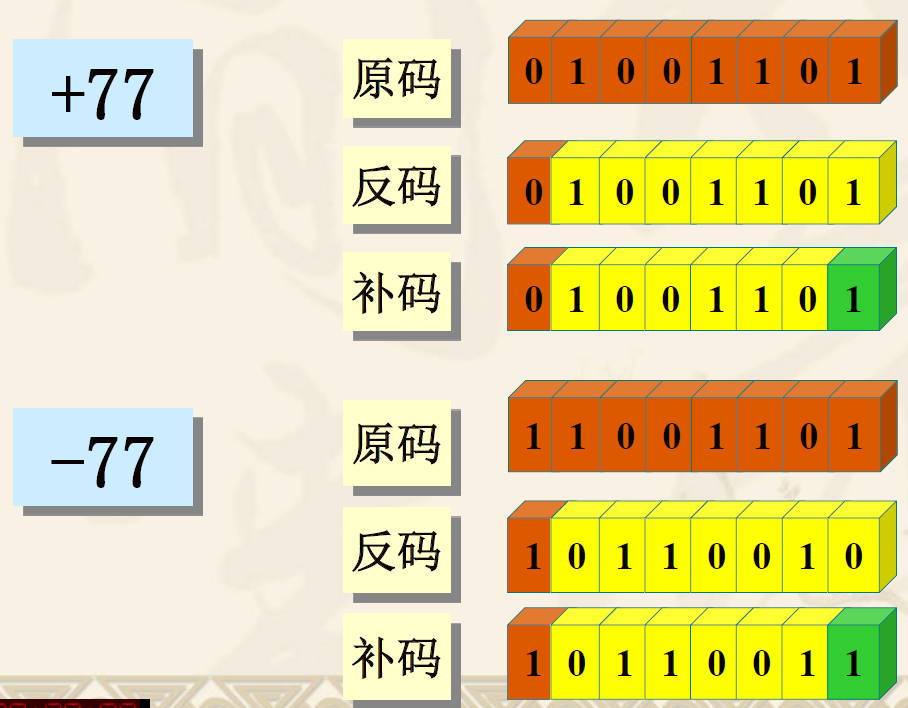
\includegraphics[scale=0.25]{2}
\end{frame}

\begin{frame}{机内以补码形式存储有符号数}
\begin{enumerate}
	\setlength{\itemsep}{.5cm}
	\item 对于正数,原码=反码=补码
	\item 对于负数,补码=反码 + 1\\
	      反码 = 符号位不变, 其他位按位取反
	\item 补码是可逆的,即再对补码求补得到原码。
	\item 引入补码后,使减法统一为加法。
	$(+77)_{\text{补}}+(-77)_{\text{补}}=0100~1101+1011~0011=0000~0000$	
\end{enumerate}
\end{frame}

\note
{
	0原码是00000000 -0原码是10000000
	
	0反码是00000000 -0反码是11111111
	
	0补码是00000000 补码没有正0与负0之分。+0和-0的补码是一样的。即 0的补码只有一种表示。
	
	+0的补码:00000000
	
	-0的补码:第一步:11111111 第二步+1= 1 00000000 第三部:进位1被丢弃 您明白了吗?
	
	在规定中,8位二进制码能表示的反码范围是-127~127。
	
	此时(字长为8位), -128没有原码和反码(只有补码)。
	
	那么,为什么规定字长8位时-128没有原码和反码呢?下面解释。
	
	首先看-0,[-0]原码=1000 000,其中1是符号位,求反操作,算出[-0]反码=1111 1111,
	
	再看-128,假如它有原码且[-128]原码=1000~000,假如让-128也有反码,求反操作,则[-128]反码=1111~1111,
	
	你会发现,-128的反码和-0的反码相同,所以为了避免面混淆,有了-0的原码,便不能有-128的原码补码,这是8位比特位位数限制决定的。
}

\begin{frame}{补码运算实例(以8bit编码为例)}
\textcolor{blue}{补码可逆:}
\begin{align*}
&[-25]_{\text{原}}=(1001~1001)_2\quad [-25]_{\text{反}}=(1110~0110)_2\\
&[-25]_{\text{补}}=[-25]_{\text{反}}+1=(1110~0110+1)_2=(1110~0111)_2\\
&[-25]_{\text{原}}=\left([-25]_{\text{补}}\right)_{\text{补}}=(1001~1000+1)_2=(1001~1001)_2
\end{align*}

\textcolor{blue}{减法统一为加法: $[a-b]_{\text{补}}=a_{\text{补}}+[-b]_{\text{补}}$}
\begin{align*}
&[102-25]_{\text{补}}=[77]_{\text{补}}=(0100~1101)_2=77\\
&[102]_{\text{补}}+[-25]_{\text{补}}=(0110~0110)_2+(1110~0111)_2=(0100~1101)_2=77\\
&\text{所以, }[102-25]_{\text{补}}=[102]_{\text{补}}+[-25]_{\text{补}}\\
&\text{同样有, }[25-102]_{\text{补}}=[25]_{\text{补}}+[-102]_{\text{补}}\\
\end{align*}
\end{frame}

\begin{frame}{ASCII编码表$B_6B_5B_4B_3B_2B_1B_0$}
\begin{columns}
	\column{0.65\textwidth}
	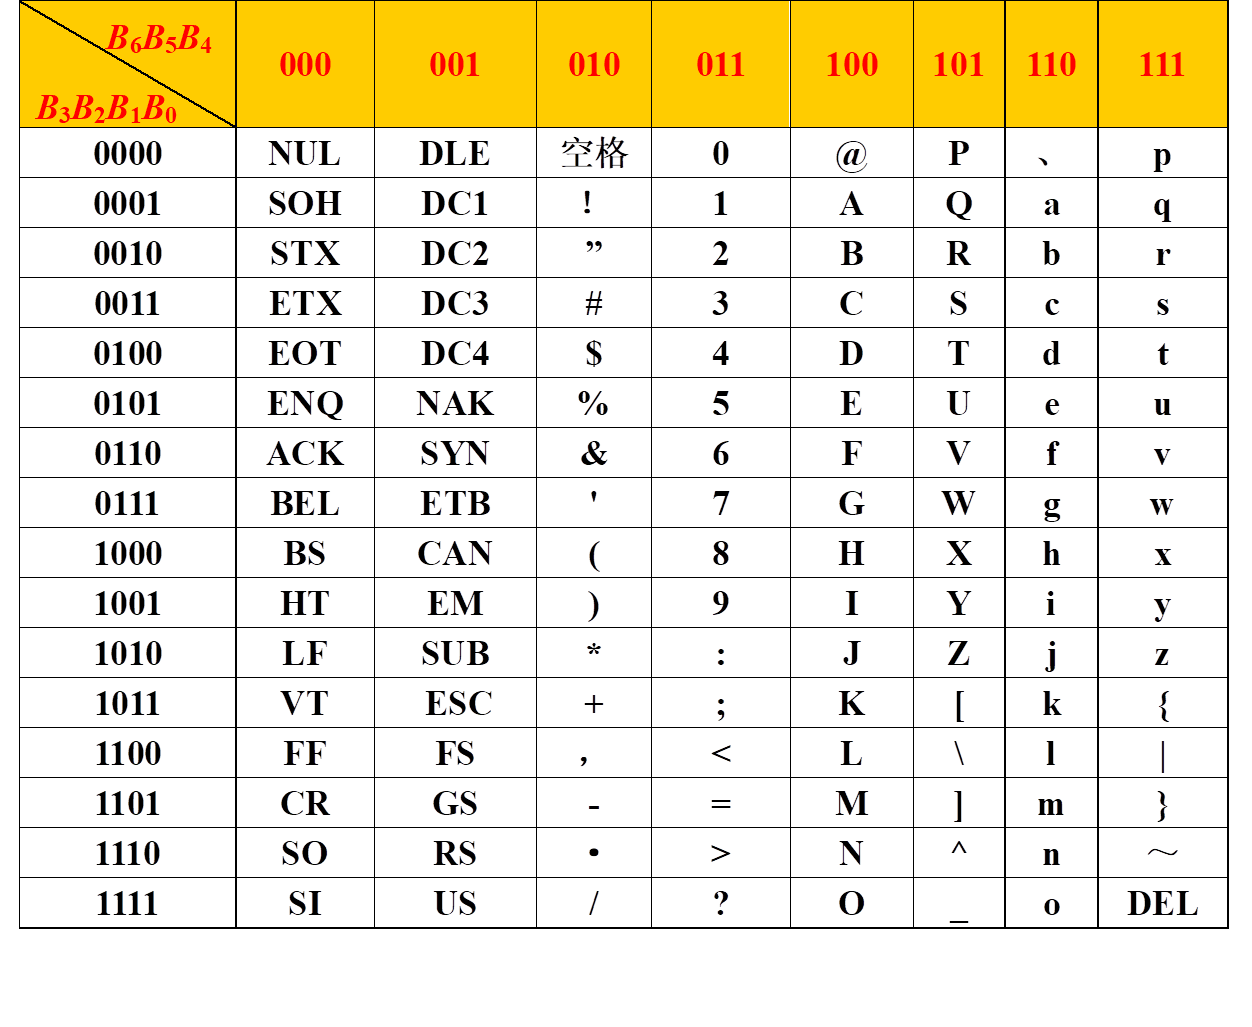
\includegraphics[scale=0.4]{ASCII}
	\column{0.35\textwidth}
	\begin{itemize}
		\item ASCII码连续排列 \\
		 `0'$\sim$`9', `A'$\sim$`Z', `a'$\sim$`z'
		\item 数字 = 编码值 - `0' \\
		 9=`9'-`0'
		\item 大小字符间隔: \\
		`a' - `A' = 32
		
		\scriptsize{
		`a'=0110~0001=61H=0X61=97
		
		'A'=0100~0001=41H=0X41=65}
	\end{itemize}	
\end{columns}
\end{frame}

\section{C语言程序设计简介}

\begin{frame}{计算机程序}
\centering

\includegraphics[scale=0.4]{program1}
\end{frame}

\begin{frame}{计算机语言}
\centering
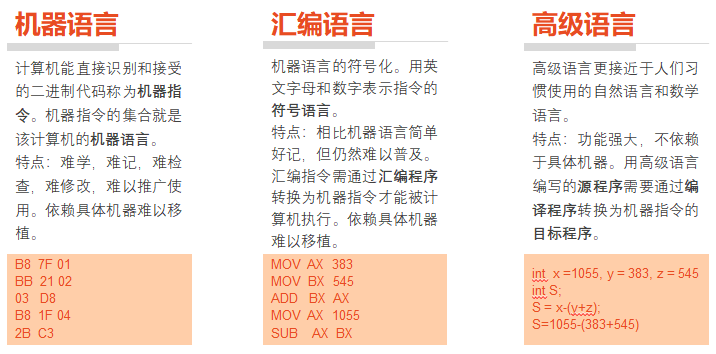
\includegraphics[scale=0.4]{program2}
\end{frame}

\begin{frame}{高级语言的发展}
\centering
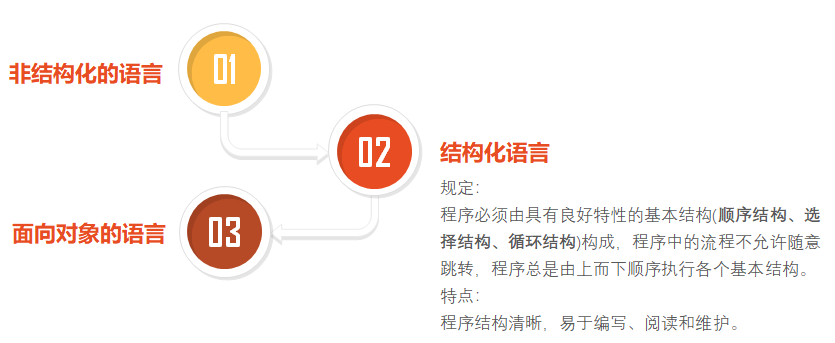
\includegraphics[scale=0.4]{program3}
\end{frame}

\begin{frame}{C语言的特点}
\vspace{-0.5cm}
\begin{enumerate}
	\item 语言简洁、紧凑,使用方便、灵活
    \item 运算符丰富
    \item 数据类型丰富
    \item \textcolor{blue}{C语言是完全模块化和结构化的语言}\\
          具有结构化的控制语句(顺序、选择、循环结构)\\
          用函数作为程序的模块单位,便于实现程序的模块化
    \item \textcolor{blue}{兼具高级语言和低级语言的功能}\\
          允许直接访问物理地址\\
          能进行位(bit)操作\\  
          能实现汇编语言的大部分功能\\
          可以直接对硬件进行操作        
\end{enumerate}
\end{frame}

\begin{frame}{程序设计的任务}
\centering
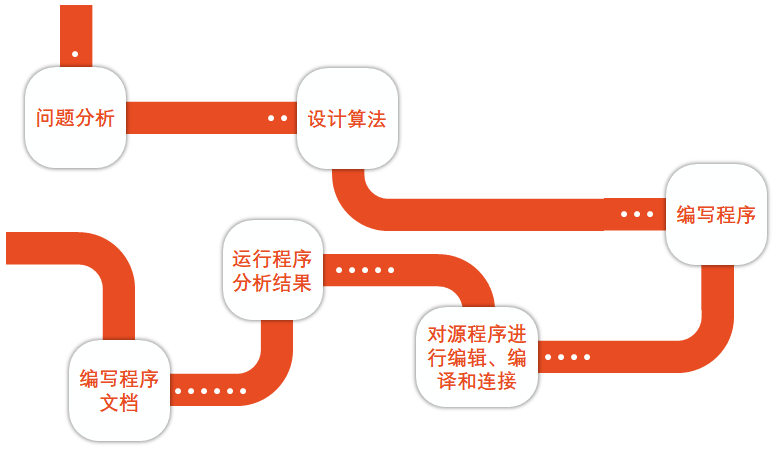
\includegraphics[scale=0.4]{program}
\end{frame}

\begin{frame}[fragile]{第一个C语言程序}
    \begin{lstlisting}
    #include<stdio.h>            // standard input/output编译预处理指令
    int main()                   // 主函数
    {                            // 函数开始标志
       printf("Hello World!");   // 输出一行信息
       return 0;                 // 函数执行完毕返回函数值0
    }                            // 函数结束标志
    \end{lstlisting}
\end{frame}

\begin{frame}[fragile]{求两个整数之和}
\begin{lstlisting}
#include<stdio.h>         // standard input/output编译预处理指令
int main()                // 主函数
{                         // 函数开始标志
   int a,b,sum;           // 定义a,b,sum为整型变量
   a=123;                 // 对a,b赋值
   b=456;
   sum=a+b;               // 计算a+b, 并把结果存放在变量sum中
   printf("sum is %d\n",sum);// 输出结果
   return 0;                 // 函数执行完毕返回函数值0
}                            // 函数结束标志
\end{lstlisting}
\end{frame}
